%
%

\section{How to buld a quantum computer?}
\chapterframe{How to build a quantum computer?}


\begin{frame}{Requirements for a quantum computer}
 \begin{itemize}
   \item A scalable physical system with well characterized quibits
    \item The ability to initialize the state of the qubits to a simple fiducial state such as $\bra{000\dots}$
    \item Long relevant decoherence times, much longer than the gate operation time
    \item A "universal" set of quantum gates
    \item A qubit-specific measurement capability
 
 \end{itemize}
\end{frame}

\begin{frame}{Problems}

 \begin{itemize}
 
  \item \textbf{Relaxation} - falling back to state with lower energy.
  
  \item \textbf{Dekoherence} - superposition gets lost through external influence.
 
 \end{itemize}


\end{frame}

\begin{frame}{Possible Technological Candiates}
 \begin{itemize}
  \item Bose-Einstein condensate (BEC)
  \item Ion Traps
  \item Super-conducting qubits
  \item Cold-atom optical lattices
  \item NV-centers in diamonds
  \item Semiconductor quantum dots
 \end{itemize}

\end{frame}

\begin{frame}{Bose-Einstein condensate (BEC)}

\begin{itemize}
  \item Temperature very close to 0 K
  \item Quantum effects manifest on macroscopic level
  \item Same quantum state over multiple atom
  \item Two-component BCE for qubits.
\end{itemize}


\end{frame}

\begin{frame}{Ion Traps}

\begin{itemize}
	\item Long storage of state
    \item Ions in vacuum 
    \item Initialisation with optical pumping
    \item Measurement via laser
    \item Operations 97\% successful
\end{itemize}    
    
\end{frame}


\begin{frame}{Super-conducting qubits}

\begin{itemize}
 \item Super-conducting circuit
 \item With Josephson junction
 \item Initialisation with microwaves
 
\end{itemize}

\end{frame}

\begin{frame}{Cold-atom in opcial lattices}

\begin{itemize}
 \item Grid of laser beams
 \item Periodic potential traps neutral atoms

\end{itemize}

	\begin{center}
		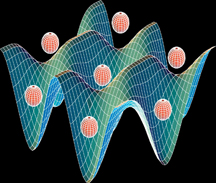
\includegraphics[scale=0.8]{optlat.jpg}
	\end{center}


\end{frame}


\begin{frame}{NV-centers in diamonds}

\begin{itemize}
 \item Nitrogen (N) replaces carbon (C) in diamond
 \item Initialisation with laser beams
 \item Diamond structure isolates qubits from external influence
 \item No cooling required
\end{itemize}

\end{frame}


\begin{frame}{Semiconductor quantum dot}

\begin{itemize}
  \item $10^3$ to $10^9$ atoms
  \item Electrons cannot move
  \item Discrete electronic state
  \item Qubit as spin of electron
  \item Initialisation with magnetic fields  
\end{itemize}


\end{frame}

\section{Recent developments}
\chapterframe{Recent developments}

\begin{frame}{Recent developments}
%(neue papers)

	\begin{itemize}
 		\item At the TU:
        	\begin{itemize}
            	\item \url{http://www.tuwien.ac.at/aktuelles/news_detail/article/8744/}
            \end{itemize}
     \end{itemize}


\end{frame}